\documentclass[14pt, oneside]{altsu-report}

\usepackage{totcount}
\usepackage{svg}

\worktype{Отчёт по технологической (проектно-технологической) практике на тему:}
\title{Рост дендрита}
\author{М.\,Е.~Пивоваров}
\groupnumber{5.205-1}
\GradebookNumber{1337}
\supervisor{И.\,А.~Шмаков}
\supervisordegree{преп.}
\ministry{Министерство науки и высшего образования}
\country{Российской Федерации}
\fulluniversityname{ФГБОУ ВО Алтайский государственный университет}
\institute{Институт цифровых технологий, электроники и физики}
\department{Кафедра вычислительной техники и электроники}
\departmentchief{В.\,В.~Пашнев}
\departmentchiefdegree{к.ф.-м.н., доцент}
\shortdepartment{ВТиЭ}
\abstractRU{
Данная работа посвещена разработке программы на языке программирования Python с использованием библиотеки FLTK, моделирующую рост дендрита.

Целью работы является создание программы на языке программирования Python с использованием библиотеки FLTK, моделирующую рост дендрита.

В работе рассмотрены теоретические сведения о дендрите и его росте, о библиотеке FLTK, языке программирования Python, среде разработки Geany. Практические сведения о ходе разработки программы "Рост дендрита".
}
\abstractEN{Большой текст на английском!}
\keysRU{дендрит, частица, функция, моделирование}
\keysEN{computer simulation, distributed version control}
\countWorkPage{21}
\countWorkImg{3}
\countWorkLit{8}
\countWorkTab{0}

\date{\the\year}

% Подключение файлов с библиотекой.
\addbibresource{graduate-students.bib}

% Пакет для отладки отступов.
%\usepackage{showframe}

\begin{document}
\maketitle

\setcounter{page}{2}
\makeabstract
\tableofcontents

\chapter*{Введение}
\phantomsection\addcontentsline{toc}{chapter}{ВВЕДЕНИЕ}

\textbf{Актуальность}
Актуальность обусловлена непрерывном совершенствованием информационных технологий и обновлением информационных систем. Программные обеспечения используются во многих сферах человеческой деятельности.
Написание своей собственной программы является важной частью обучения навыкам программирования. А обучение навыкам программирования в свою очередь является важной частью моего направления подготовки. 

\textbf{Цель}

Создать программу на языке Python с использованием библиотеки FLTK, моделирующую рост дендрита с возможностью настроек различных параметров.

\textbf{Задачи:}
\begin{enumerate}
\item Установить библиотеку FLTK.
\item Выбрать редактор для разработки программы.
\item Изучить библиотеку FLTK.
\item Написать программу.
\end{enumerate}

% Подключение первой главы (теория):
\chapter{\label{ch:ch01}ТЕОРЕТИЧЕСКАЯ ЧАСТЬ} % Нужно сделать главу в содержании заглавными буквами

\section{Дендрит}
\textbf{Дендри́ты}~\cite{wikiDen} (от греч. δένδρον — дерево) — сложнокристаллические образования древовидной ветвящейся структуры.
\subsubsection{Формирование} %не нужен секшен
Дендрит представляет собой ветвящееся и расходящееся в стороны образование, возникающее при ускоренной или стеснённой кристаллизации в неравновесных условиях, когда кристалл расщепляется по определённым законам. В результате он утрачивает свою первоначальную целостность, появляются кристаллографически разупорядоченные блоки. Они ветвятся и разрастаются в разные стороны подобно дереву, тянущемуся к солнечному свету, кристаллографическая закономерность изначального кристалла в процессе его дендритного развития утрачивается по мере его роста. Дендриты могут быть трёхмерными объёмными (в открытых пустотах) или плоскими двумерными (если растут в тонких трещинах горных пород).

Процесс образования дендрита принято называть дендритный рост.

Самый крупный дендрит был обнаружен в конце XIX века в 100-тонном слитке стали и был назван в честь русского учёного Дмитрия Константиновича Чернова, детально исследовавшего процесс зарождения и роста кристаллов (в частности, дендритных стальных кристаллов). Вес «кристалла Д. К. Чернова» составил 3,45 кг, длина — 39 см, химический состав — 0,78 \% углерода, 0,255 \% кремния, 1,055 \% марганца, 97,863 \% железа.
\subsubsection{Разновидности}
В качестве примера дендритов можно привести снежинки, ледяные узоры на оконном стекле, живописные окислы марганца, имеющие вид деревьев в пейзажных халцедонах («моховой агат») и в тонких трещинах розового родонита. Другие примеры — веточки самородной меди в зонах окисления рудных месторождений, дендриты самородных серебра и золота, решётчатые дендриты самородного висмута и ряда сульфидов. Почковидные или кораллообразные дендриты известны для малахита, барита и многих других минералов, к ним относятся и так называемые «пещерные цветы» кальцита и арагонита в карстовых пещерах.
\section{FLTK} %обзор
Fast, Light Toolkit~\cite{wikiFL} — кросс-платформенная библиотека инструментов с открытым исходным кодом (лицензия LGPL) для построения графического интерфейса пользователя (GUI). FLTK произносится как «фултик».

Изначально разрабатывалась Биллом Спицтаком (Bill Spiztak). FLTK создавалась для поддержки 3D графики и поэтому имеет встроенный интерфейс к OpenGL, но хорошо подходит и для программирования обычных интерфейсов пользователя.

Библиотека использует свои собственные независимые системы виджетов, графики и событий, что позволяет писать программы одинаково выглядящие и работающие на разных операционных системах. В отличие от других подобных библиотек (Qt, GTK, wxWidgets) FLTK ограничивается только графической функциональностью. Поэтому она имеет малый размер и обычно компонуется статически (это исключение из лицензии GNU Lesser General Public License, разрешенное разработчиками). FLTK не использует сложных макросов, препроцессоров и продвинутых возможностей языка C++ (шаблоны, исключения, пространства имен). Вкупе с малым размером кода, это облегчает использование библиотеки не очень искушенными пользователями.

Однако эти достоинства порождают недостатки библиотеки, такие как меньшее число виджетов, несколько упрощенная графика и невозможность сборки приложения, выглядящего естественно под конкретной операционной системой.
\subsubsection{Название}
Изначально назывался FL (Forms Library). При переходе в open source выяснилось, что поиск по названию FL практически невозможен — аббревиатура FL также означает штат Флорида. Поэтому пакет был переименован в FLTK (FL Toolkit), позднее ему был придуман бэкроним Fast, Light Toolkit.
\subsubsection{История}
FLTK начал разрабатываться как замена библиотеке XForms, а позднее был портирован на Mac OS и Windows. FLTK появился раньше, чем другие популярные библиотеки для создания GUI, но был практически неизвестен до 1998 года.
\subsubsection{Особенности}
FLTK представляет собой библиотеку виджетов и работает на ОС UNIX/Linux X11, Microsoft Windows и MacOS X. Малый объём библиотеки делает её подходящей для использования во встраиваемых системах.

Для встраиваемых систем на основе embedded Linux возможны следующие варианты:

FLTK + nxlib + nano-X (довольно стабильно работает, но есть проблемы с кириллицей)

FLNX — порт FLTK 1.0.7 на nano-X (работает только с версией 0.92)

DirectFB FLTK — порт FLTK на DirectFB + собственно сам DirectFB (данная сборка нестабильная, шрифты необходимо инсталлировать как для X11 и указать путь в конфиге)

\section{Visual Studio Code}
\textbf{Visual Studio Code} (VS Code)~\cite{wikiVS} — текстовый редактор, разработанный Microsoft для Windows, Linux и macOS. Позиционируется как «лёгкий» редактор кода для кроссплатформенной разработки веб- и облачных приложений. Включает в себя отладчик, инструменты для работы с Git, подсветку синтаксиса, IntelliSense и средства для рефакторинга. Имеет широкие возможности для кастомизации: пользовательские темы, сочетания клавиш и файлы конфигурации. Распространяется бесплатно, разрабатывается как программное обеспечение с открытым исходным кодом, но готовые сборки распространяются под проприетарной лицензией.

Visual Studio Code основан на Electron и реализуется через веб-редактор Monaco, разработанный для Visual Studio Online.
\subsubsection{История}
Visual Studio Code был анонсирован 29 апреля 2015 года компанией Microsoft на конференции Build, и вскоре была выпущена бета-версия.

18 ноября 2015 года Visual Studio Code был выпущен под лицензией MIT, а исходный код был опубликован на GitHub. Анонсирована поддержка расширений.

14 апреля 2016 года Visual Studio Code вышел из стадии бета-тестирования.
\subsubsection{Возможности}
Visual Studio Code — это редактор исходного кода. Он имеет многоязычный интерфейс пользователя и поддерживает ряд языков программирования, подсветку синтаксиса, IntelliSense, рефакторинг, отладку, навигацию по коду, поддержку Git и другие возможности. Многие возможности Visual Studio Code недоступны через графический интерфейс, зачастую они используются через палитру команд или JSON-файлы (например, пользовательские настройки). Палитра команд представляет собой подобие командной строки, которая вызывается сочетанием клавиш.

VS Code также позволяет заменять кодовую страницу при сохранении документа, символы перевода строки и язык программирования текущего документа.

С 2018 года появилось расширение Python для Visual Studio Code с открытым исходным кодом. Оно предоставляет разработчикам широкие возможности для редактирования, отладки и тестирования кода.

Также VS Code поддерживает редактирование и выполнение файлов типа «Блокнот Jupyter» (Jupyter Notebook) напрямую «из коробки» без установки внешнего модуля в режиме визуального редактирования и в режиме редактирования исходного кода.

На март 2019 года посредством встроенного в продукт пользовательского интерфейса можно загрузить и установить несколько тысяч расширений только в категории «programming languages» (языки программирования).

Также расширения позволяют получить более удобный доступ к программам, таким как Docker, Git и другие. В расширениях можно найти линтеры кода, темы для редактора и поддержку синтаксиса отдельных языков.

Visual Studio Code имеет поддержку плагинов, доступных через Visual Studio Marketplace. Они могут включать в себя дополнения к редактору, поддержку дополнительных языков программирования, статические анализаторы кода.

С мая 2019 года доступен закрытый тест редактора Visual Studio Online на основе VS Code. Он поддерживает все расширения и IntelliCode.
\section{Python}
Python~\cite{wikiPy} (в русском языке встречаются названия пито́н или па́йтон) — высокоуровневый язык программирования общего назначения с динамической строгой типизацией и автоматическим управлением памятью, ориентированный на повышение производительности разработчика, читаемости кода и его качества, а также на обеспечение переносимости написанных на нём программ. Язык является полностью объектно-ориентированным в том плане, что всё является объектами. Необычной особенностью языка является выделение блоков кода отступами. Синтаксис ядра языка минималистичен, за счёт чего на практике редко возникает необходимость обращаться к документации. Сам же язык известен как интерпретируемый и используется в том числе для написания скриптов. Недостатками языка являются зачастую более низкая скорость работы и более высокое потребление памяти написанных на нём программ по сравнению с аналогичным кодом, написанным на компилируемых языках, таких как C или C++.

Python является мультипарадигменным языком программирования, поддерживающим императивное, процедурное, структурное, объектно-ориентированное программирование, метапрограммирование, функциональное программирование и асинхронное программирование. Задачи обобщённого программирования решаются за счёт динамической типизации. Аспектно-ориентированное программирование частично поддерживается через декораторы, более полноценная поддержка обеспечивается дополнительными фреймворками. Такие методики как контрактное и логическое программирование можно реализовать с помощью библиотек или расширений. Основные архитектурные черты — динамическая типизация, автоматическое управление памятью, полная интроспекция, механизм обработки исключений, поддержка многопоточных вычислений с глобальной блокировкой интерпретатора (GIL), высокоуровневые структуры данных. Поддерживается разбиение программ на модули, которые, в свою очередь, могут объединяться в пакеты.

Эталонной реализацией Python является интерпретатор CPython, который поддерживает большинство активно используемых платформ, являющийся стандартом де-факто языка. Он распространяется под свободной лицензией Python Software Foundation License, позволяющей использовать его без ограничений в любых приложениях, включая проприетарные. CPython компилирует исходные тексты в высокоуровневый байт-код, который исполняется в стековой виртуальной машине. К другим трём основным реализациям языка относятся Jython (для JVM), IronPython (для CLR/.NET) и PyPy. PyPy написан на подмножестве языка Python (RPython) и разрабатывался как альтернатива CPython с целью повышения скорости исполнения программ, в том числе за счёт использования JIT-компиляции. Поддержка версии Python 2 закончилась в 2020 году. На текущий момент активно развивается версия языка Python 3. Разработка языка ведётся через предложения по расширению языка PEP (англ. Python Enhancement Proposal), в которых описываются нововведения, делаются корректировки согласно обратной связи от сообщества и документируются итоговые решения.

Стандартная библиотека включает большой набор полезных переносимых функций, начиная с возможностей для работы с текстом и заканчивая средствами для написания сетевых приложений. Дополнительные возможности, такие как математическое моделирование, работа с оборудованием, написание веб-приложений или разработка игр, могут реализовываться посредством обширного количества сторонних библиотек, а также интеграцией библиотек, написанных на Си или C++, при этом и сам интерпретатор Python может интегрироваться в проекты, написанные на этих языках[14]. Существует и специализированный репозиторий программного обеспечения, написанного на Python, — PyPI. Данный репозиторий предоставляет средства для простой установки пакетов в операционную систему и стал стандартом де-факто для Python. По состоянию на 2019 год в нём содержалось более 175 тысяч пакетов.

Python стал одним из самых популярных языков, он используется в анализе данных, машинном обучении, DevOps и веб-разработке, а также в других сферах, включая разработку игр. За счёт читабельности, простого синтаксиса и отсутствия необходимости в компиляции язык хорошо подходит для обучения программированию, позволяя концентрироваться на изучении алгоритмов, концептов и парадигм. Отладка же и экспериментирование в значительной степени облегчаются тем фактом, что язык является интерпретируемым. Применяется язык многими крупными компаниями, такими как Google или Facebook.


% Подключение второй главы (практическая часть):
\chapter{\label{ch:ch02}ГЛАВА 2}

\section{\label{sec:ch02/sec01}Раздел 1}

\subsection{\label{subsec:ch02/sec01/sub01}Подраздел 1}

Пример ссылки на рисунок в документе~\ref{fig:example03}.
\begin{figure}[h]
    \centering
    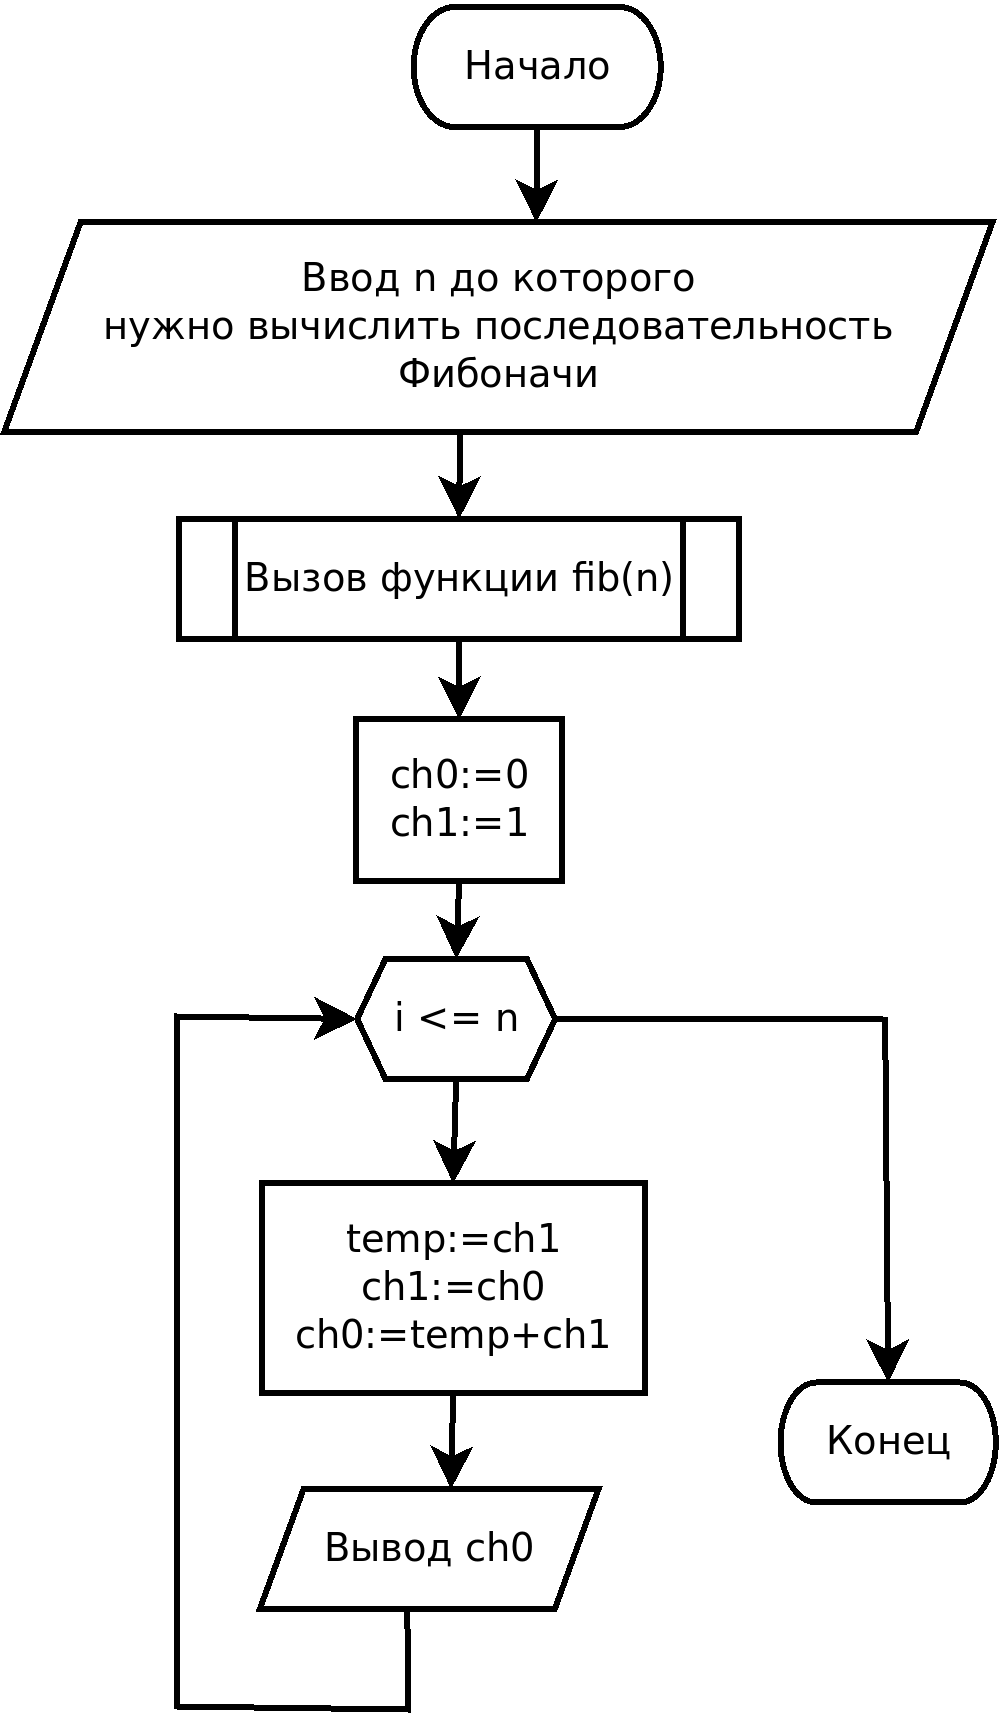
\includegraphics[width=0.5\textwidth]{./images/fibonacci.png}
    \caption{\centering\label{fig:example03}Пример рисунка в формате PNG.}
\end{figure}

Пример ссылки на рисунок в документе~\ref{fig:example04}.
\begin{figure}[h]
    \centering
    \includesvg[width=0.5\textwidth]{./images/fibonacci.svg}
    \caption{\centering\label{fig:example04}Пример рисунка в формате SVG.}
\end{figure}

\subsection{\label{subsec:ch02/sec01/sub02}Подраздел 2}

\section{\label{sec:ch02/sec02}Раздел 2}

\subsection{\label{subsec:ch02/sec02/sub01}Подраздел 1}

\subsection{\label{subsec:ch02/sec02/sub02}Подраздел 2}

Пример ссылки на таблицу в документе~\ref{tab:example03}.
\begin{table}[H]
\caption{\label{tab:example03}Системные требования}
\begin{tabular}{|p{3 cm}|p{3 cm}|p{3 cm}|p{5 cm}|}
\hline
Минимальные требования & 1 & 2 & 3 \\ \hline
Версия операционной системы & 1 & 2 & 3 \\ \hline
Процессор & 1 & 2 & 3 \\ \hline
Графический API & 1 & 2 & 3 \\ \hline
\end{tabular}
\end{table}

Пример ссылки на таблицу в документе~\ref{tab:example04}.
\begin{table}[H]
\caption{\centering\label{tab:example04}Системные требования}
\begin{tabular}{|p{3 cm}|p{3 cm}|p{3 cm}|p{5 cm}|}
\hline
Минимальные требования & 1 & 2 & 3 \\ \hline
Версия операционной системы & 1 & 2 & 3 \\ \hline
Процессор & 1 & 2 & 3 \\ \hline
Графический API & 1 & 2 & 3 \\ \hline
\end{tabular}
\end{table}

Пример использования minted для оформления кода и ссылка на этот код~\ref{code:example03}.
\begin{code}
\captionof{listing}{\centering\label{code:example03}Вычисление последовательности Фибоначчи}
\vspace{-\baselineskip}\begin{minted}{C}
#include <stdio.h>
#include <omp.h>
#define N 100

int main(int argc, char *argv[]) {
  double a[N], b[N], c[N];
  int i;
  omp_set_dynamic(0); // запретить библиотеке openmp менять число потоков во время исполнения
  omp_set_num_threads(10); // установить число потоков в 10
  // инициализируем массивы
  for (i = 0; i < N; i++) {
      a[i] = i * 1.0;
      b[i] = i * 2.0;
  }
  // вычисляем сумму массивов
#pragma omp parallel for shared(a, b, c) private(i)
   for (i = 0; i < N; i++)
     c[i] = a[i] + b[i];

  printf ("%f\n", c[10]);
  return 0;
}
\end{minted}
\end{code}

Пример использования minted для оформления кода и ссылка на этот код~\ref{code:example04}.
\begin{code}
\captionof{listing}{\centering\label{code:example04}Сложение двух массивов параллельно десятью потоками (пример из https://ru.wikipedia.org/wiki/OpenMP)}
\vspace{-\baselineskip}\begin{minted}{C}
#include <stdio.h>
#include <omp.h>
#define N 100

int main(int argc, char *argv[]) {
  double a[N], b[N], c[N];
  int i;
  omp_set_dynamic(0); // запретить библиотеке openmp менять число потоков во время исполнения
  omp_set_num_threads(10); // установить число потоков в 10
  // инициализируем массивы
  for (i = 0; i < N; i++) {
      a[i] = i * 1.0;
      b[i] = i * 2.0;
  }
  // вычисляем сумму массивов
#pragma omp parallel for shared(a, b, c) private(i)
   for (i = 0; i < N; i++)
     c[i] = a[i] + b[i];

  printf ("%f\n", c[10]);
  return 0;
}
\end{minted}
\end{code}

% Подключение третий главы (практическая часть с тестированием:
% \chapter{\label{ch:ch03}ГЛАВА 3}

Пример ссылок:
\begin{enumerate}
\item на главу~\ref{ch:ch01};
\item на раздел~\ref{sec:ch01/sec01} главы~\ref{ch:ch01};
\item на раздел~\ref{sec:ch02/sec01} главы~\ref{ch:ch02};
\item на приложение на странице~\pageref{appendix1};
\item на код на странице~\pageref{code:pi-example}.
\end{enumerate}

\section{\label{sec:ch03/sec01}Раздел 1}

\subsection{\label{subsec:ch03/sec01/sub01}Подраздел 1}

\subsection{\label{subsec:ch03/sec01/sub02}Подраздел 2}

\section{\label{sec:ch03/sec02}Раздел 2}

\subsection{\label{subsec:ch03/sec02/sub01}Подраздел 1}

\subsection{\label{subsec:ch03/sec02/sub02}Подраздел 2}

Пример ссылки на рисунок в документе~\ref{fig:example05}.
\begin{figure}[h]
    \centering
    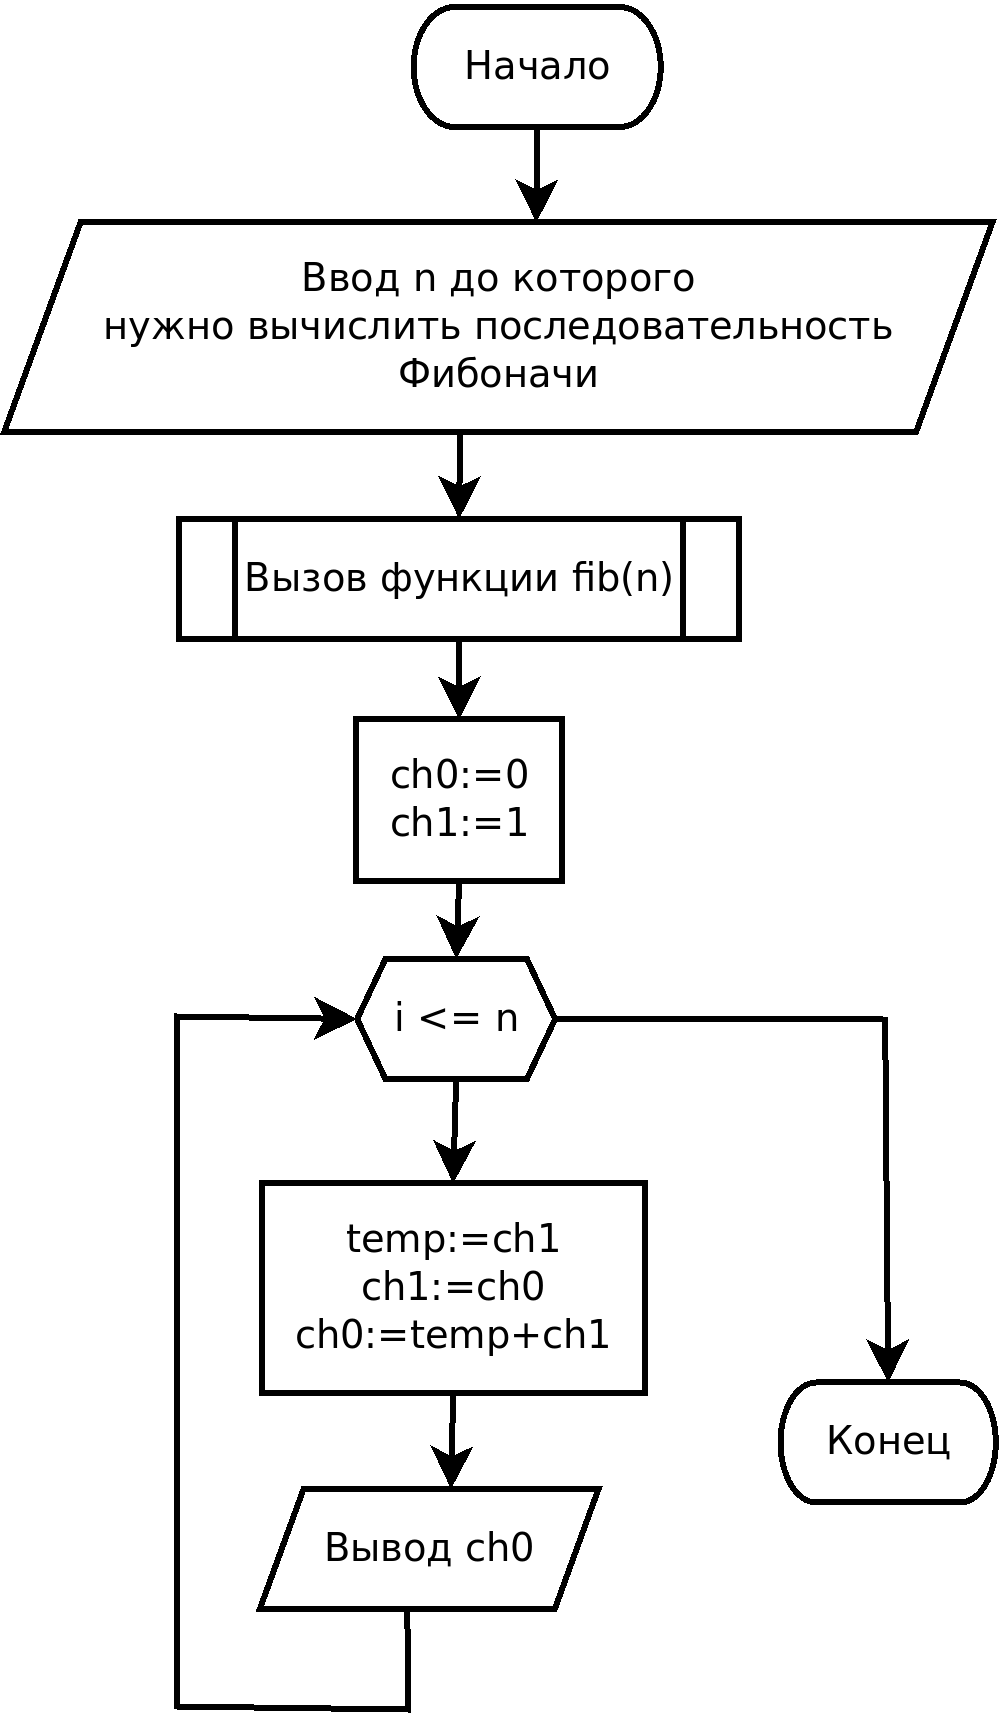
\includegraphics[width=0.5\textwidth]{./images/fibonacci.png}
    \caption{\centering\label{fig:example05}Пример рисунка в формате PNG.}
\end{figure}

Пример ссылки на рисунок в документе~\ref{fig:example06}.
\begin{figure}[h]
    \centering
    \includesvg[width=0.5\textwidth]{./images/fibonacci.svg}
    \caption{\centering\label{fig:example06}Пример рисунка в формате SVG.}
\end{figure}

Пример ссылки на таблицу в документе~\ref{tab:example05}.
\begin{table}[H]
\caption{\centering\label{tab:example05}Системные требования}
\begin{tabular}{|p{3 cm}|p{3 cm}|p{3 cm}|p{5 cm}|}
\hline
Минимальные требования & 1 & 2 & 3 \\ \hline
Версия операционной системы & 1 & 2 & 3 \\ \hline
Процессор & 1 & 2 & 3 \\ \hline
Графический API & 1 & 2 & 3 \\ \hline
\end{tabular}
\end{table}

Пример ссылки на таблицу в документе~\ref{tab:example06}.
\begin{table}[H]
\caption{\centering\label{tab:example06}Системные требования}
\begin{tabular}{|p{3 cm}|p{3 cm}|p{3 cm}|p{5 cm}|}
\hline
Минимальные требования & 1 & 2 & 3 \\ \hline
Версия операционной системы & 1 & 2 & 3 \\ \hline
Процессор & 1 & 2 & 3 \\ \hline
Графический API & 1 & 2 & 3 \\ \hline
\end{tabular}
\end{table}

Пример использования minted для оформления кода и ссылка на этот код~\ref{code:example05}.
\begin{code}
\captionof{listing}{\centering\label{code:example05}Вычисление последовательности Фибоначчи}
\vspace{-\baselineskip}\begin{minted}{C}
#include <stdio.h>
#include <omp.h>
#define N 100

int main(int argc, char *argv[]) {
  double a[N], b[N], c[N];
  int i;
  omp_set_dynamic(0); // запретить библиотеке openmp менять число потоков во время исполнения
  omp_set_num_threads(10); // установить число потоков в 10
  // инициализируем массивы
  for (i = 0; i < N; i++) {
      a[i] = i * 1.0;
      b[i] = i * 2.0;
  }
  // вычисляем сумму массивов
#pragma omp parallel for shared(a, b, c) private(i)
   for (i = 0; i < N; i++)
     c[i] = a[i] + b[i];

  printf ("%f\n", c[10]);
  return 0;
}
\end{minted}
\end{code}

Пример использования minted для оформления кода и ссылка на этот код~\ref{code:example06}.
\begin{code}
\captionof{listing}{\centering\label{code:example06}Сложение двух массивов параллельно десятью потоками (пример из https://ru.wikipedia.org/wiki/OpenMP)}
\vspace{-\baselineskip}\begin{minted}{C}
#include <stdio.h>
#include <omp.h>
#define N 100

int main(int argc, char *argv[]) {
  double a[N], b[N], c[N];
  int i;
  omp_set_dynamic(0); // запретить библиотеке openmp менять число потоков во время исполнения
  omp_set_num_threads(10); // установить число потоков в 10
  // инициализируем массивы
  for (i = 0; i < N; i++) {
      a[i] = i * 1.0;
      b[i] = i * 2.0;
  }
  // вычисляем сумму массивов
#pragma omp parallel for shared(a, b, c) private(i)
   for (i = 0; i < N; i++)
     c[i] = a[i] + b[i];

  printf ("%f\n", c[10]);
  return 0;
}
\end{minted}
\end{code}


\chapter*{Заключение}
\phantomsection\addcontentsline{toc}{chapter}{ЗАКЛЮЧЕНИЕ}

В результате выполнения работы ее цель была достигнута. Была изучена библиотека FLTK и получен опыт работы с ней. Получено больше опыта написания кода на языке программирования Python, написания отчета с помощью Latex, написания программы с графическим интерфейсом. В итоге была разработана программа, моделирующая рост дендрита с возможностью настройки различных параметров и также было успешно проведено ее тестирование.

%\begin{enumerate}
%\item Пример ссылки на электронный источник~\cite{wikiRUBitbucket,wikiRUIdSoftware,wikiRUGitHub}.
%\item Пример ссылки на книгу одного автора~\cite{wikiFL}.
%\item Пример ссылки на книгу 5-ти и более авторов~\cite{book5author}.
%\end{enumerate}

\newpage
\phantomsection\addcontentsline{toc}{chapter}{СПИСОК ИСПОЛЬЗОВАННОЙ ЛИТЕРАТУРЫ}
\printbibliography[title={СПИСОК ИСПОЛЬЗОВАННОЙ ЛИТЕРАТУРЫ}]

\appendix
\newpage
\chapter*{\raggedleft\label{appendix1}Приложение}
\phantomsection\addcontentsline{toc}{chapter}{ПРИЛОЖЕНИЕ}
%\section*{\centering\label{code:appendix}Текст программы}

\begin{center}
\label{code:appendix}Текст программы
\end{center}

\begin{code}
\captionof*{listing}{\centering\label{code:pi-example}}
\vspace{-1cm}\inputminted{py}{src/dendrite_v3_1.py}
\end{code}

\end{document}

